\documentclass[twoside]{article}
\usepackage{amsgen,amsmath,amstext,amsbsy,amsopn,amssymb,}
\usepackage{graphicx}
\usepackage{epsfig}

\setlength{\oddsidemargin}{0.1 in} \setlength{\evensidemargin}{-0.1
in} \setlength{\topmargin}{-0.6 in} \setlength{\textwidth}{6.5 in}
\setlength{\textheight}{10 in} \setlength{\headsep}{0.1 in}
\setlength{\parindent}{0 in} \setlength{\parskip}{0.1 in}

\newcommand{\homework}[2]{
   \pagestyle{myheadings}
   \thispagestyle{plain}
   \newpage
   \setcounter{page}{1}
   \noindent
   \begin{center}
   \framebox{
      \vbox{\vspace{2mm}
       \hbox to 6.28in { {\bf Math 4720:~Statistical Methods \hfill} }
       \vspace{6mm}
       \hbox to 6.28in { {\Large \hfill #1 (#2)  \hfill} }
       \vspace{6mm}
      \vspace{2mm}}
   }
   \end{center}
   \markboth{#1}{#1}
   \vspace*{4mm}
}

\newcommand{\bbF}{\mathbb{F}}
\newcommand{\bbX}{\mathbb{X}}
\newcommand{\bI}{\mathbf{I}}
\newcommand{\bX}{\mathbf{X}}
\newcommand{\bY}{\mathbf{Y}}
\newcommand{\bepsilon}{\boldsymbol{\epsilon}}
\newcommand{\balpha}{\boldsymbol{\alpha}}
\newcommand{\bbeta}{\boldsymbol{\beta}}
\newcommand{\0}{\mathbf{0}}

\begin{document}

\homework{$1^{st}$ and $2^{nd}$ Weeks Summary}{09/07/18}
\begin{itemize}
\item What is statistics?
\item Population vs Sample.
\item Observational studies vs Experiments
\item Individuals and variables
\item Confunding variable
\item Two types of data: categorical [Nominal and Ordinal] and quantitative [Continuous and Discrete]
\item Ways to chart categorical data: frequency table, bar graphs and pie charts
\item Ways to chart quantitative data: histograms, box-plots
\item Measure of the center
\subitem Mean : $\bar{x}=\dfrac{1}{n}\sum_{i=1}^nx_i$
\subitem Median :
\item Five number summary : Min, Q1, Median, Q3, Max
\item Measure of Spread
\subitem Variance : $s^2=\dfrac{1}{n-1}\sum_{i=1}^n(x_i-\bar{x})^2$, Standard deviation : $s=\sqrt{s^2}$
\subitem IQR : $IQR = Q3 - Q1$
\item What is outlier?
\item Explanatory and response variables
\item Relationship between two variables :
\subitem Comparing data using box-plot\hspace{2in}

\begin{figure}[h]
\begin{center}
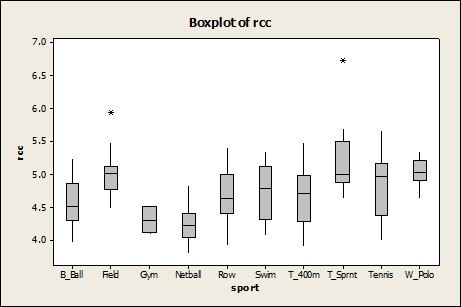
\includegraphics[angle=0,width=4.5in] {sbs_box_plot.jpg}
\end{center}
\end{figure}

\item Relationship between two variables :
\subitem Categorical vs. Quantitative : side-by-side box-plot
\subitem Quantitative vs. Quantitative : correlation $r=\dfrac{1}{n-1}\sum_{i=1}^n\Biggl(\dfrac{x_i-\bar{x}}{s_x}\Biggr)\Biggl(\dfrac{y_i-\bar{y}}{s_y}\Biggr)$
\item Properties of the Correlation r:
\subitem Takes values between $-1$ and $1$
\subitem $r = 1$ or $r = -1$ implies that the points lie on a straight line
\subitem $r = 0$ implies that there is no \textbf{linear} association
\subitem $r < 0$ implies that there is a negative \textbf{linear} association \& $r > 0$ implies positive \textbf{linear} association
\subitem If the x and y variables are switched, the correlation will stay the same
\subitem r does not change when we change the units of measurement of $x, y$, or both.
\subitem r is strongly affected by a few outliers.

\end{itemize}
\end{document}
